\documentclass{article}
\usepackage{graphicx}
\usepackage[utf8]{inputenc}
\usepackage[T1]{fontenc}
\usepackage{fouriernc}
\usepackage[margin=1in]{geometry}
\usepackage{amsmath}
\DeclareUnicodeCharacter{2212}{-}
\begin{document}

\begin{titlepage}
	\centering 
	\scshape
	\vspace*{\baselineskip}
	\rule{\textwidth}{1.6pt}\vspace*{-\baselineskip}\vspace*{2pt}
	\rule{\textwidth}{0.4pt} 
	\vspace{0.75\baselineskip}
	
	{\Large CS 374 : Computational and Numerical Methods \\\vspace{0.75\baselineskip} Set 3}
	\vspace{0.75\baselineskip}
	
	\rule{\textwidth}{0.4pt}\vspace*{-\baselineskip}\vspace{3.2pt} 
	\rule{\textwidth}{1.6pt}
	
	\vspace{2\baselineskip}  
	The Bisection Method
	
	\vspace*{3\baselineskip}
	
	\vspace{0.5\baselineskip} %originally 0.5
	
	{\scshape\large Purvil Mehta (201701073) \\ Bhargey Mehta (201701074) \\} 
	
	\vspace{1\baselineskip} 
	
	\textit{Dhirubhai Ambani Institute of Information and Communication Technology \\ Gandhinagar\\} 
	\vspace*{2\baselineskip}
	\today


\end{titlepage}

\newpage
\tableofcontents
\newpage
{\Large{\begin{center}The Bisection Method\end{center}}}

In mathematics, the bisection method is a root-finding method that applies to any continuous functions for which one knows two values with opposite signs. The method consists of repeatedly bisecting the interval defined by these values and then selecting the sub interval in which the function changes sign, and therefore must contain a root.It is a very simple and robust method, but it is also relatively slow.
\section{$f(x)$ = $x^6 - x - 1$}
We observe that $f(1) = 1^6-1-1 = -1$ and at 2, $f(2) = 2^6-2-1 = 61$, it blows up. Hence the positive root lies between 1 and 2.
\\We again see that at 0, $f(0) = -1$ and at -1, $f(-1) = 1$. Hence the negative root lies between -1 and 0.

\subsection{Plots}
\begin{figure}[!h]
    \centering
    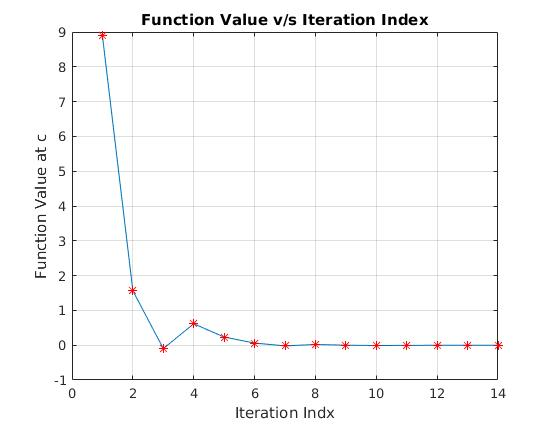
\includegraphics[scale = 0.4]{x6-x-1_1_value.jpg}
    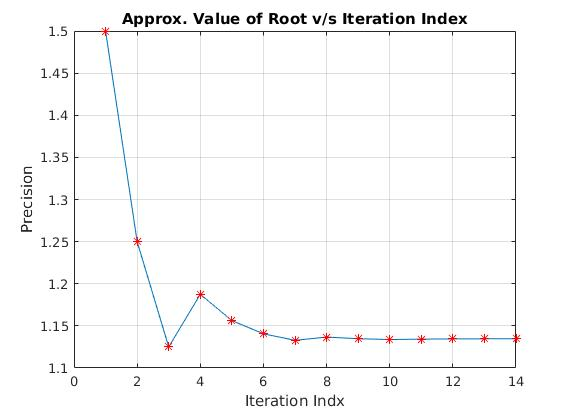
\includegraphics[scale = 0.4]{x6-x-1_root1.jpg}
    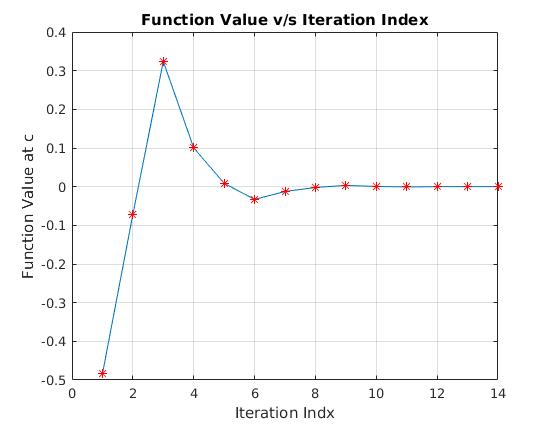
\includegraphics[scale = 0.4]{x6-x-1_2_value.jpg}
    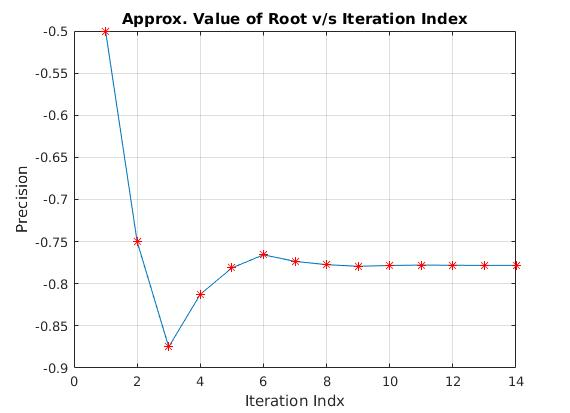
\includegraphics[scale = 0.4]{x6-x-1_root2.jpg}
    \caption{Fig 1.1,1.2 : Positive root of $x^6 - x -1 = 0$ 
     || Fig 1.3,1.4 : Negative root of $x^6 - x -1 = 0$}
    \label{fig:ques1}
\end{figure}
\newpage
\subsection{Tables}



\begin{table}[!h]
\centering{\Large
\begin{tabular}{|c|c|c|c|c|c|c|c|}\hline
ItrNo & a      & b      & c      & f(c)    & f(a)*f(c) & a-c=b-c & Assign \\ \hline
1       & 1      & 2      & 1.5    & 8.8906  & <0        & 0.5  & Set b=c   \\
2       & 1      & 1.5    & 1.25   & 1.5647  & <0        & 0.25 & Set b=c   \\
3       & 1      & 1.25   & 1.125  & -0.0977 & >0         & 0.125 & Set a=c  \\
4       & 1.125  & 1.25   & 1.1875 & 0.6167  & <0        & 0.0625 & Set b=c \\
5       & 1.125  & 1.1875 & 1.1563 & 0.2333  & <0        & 0.0313 & Set b=c \\
6       & 1.125  & 1.1563 & 1.1406 & 0.0616  & <0        & 0.0156  & Set b=c\\
7       & 1.125  & 1.1406 & 1.1328 & -0.0196 & >0         & 0.0078 & Set a=c \\
8       & 1.1328 & 1.1406 & 1.1367 & 0.0206  & <0        & 0.0039  & Set b=c\\
9       & 1.1328 & 1.1367 & 1.1348 & 0.0004  & <0        & 0.002   & Set b=c\\
10      & 1.1328 & 1.1348 & 1.1338 & -0.0096 & >0         & 0.001  & Set a=c \\
11      & 1.1338 & 1.1348 & 1.1343 & -0.0046 & >0         & 0.0005 & Set a=c \\
12      & 1.1343 & 1.1348 & 1.1345 & -0.0021 & >0         & 0.0002 & Set a=c \\
13      & 1.1345 & 1.1348 & 1.1346 & -0.0008 & >0         & 0.0001 & Set a=c \\
14      & 1.1346 & 1.1348 & 1.1347 & -0.0002 & >0         & 0.0001 & Set a=c\\    
\hline
\end{tabular}}
\caption{Positive Root of $x^6 - x - 1 =0$}
\end{table}


\begin{table}[!h]
\centering{\Large
\begin{tabular}{|c|c|c|c|c|c|c|c|}\hline
ItrNo & a      & b      & c      & f(c)    & f(a)*f(c) & a-c=b-c & Assign\\ \hline
1       & -1      & 0       & -0.5    & -0.4844 & <0        & 0.5  & Set b=c   \\
2       & -1      & -0.5    & -0.75   & -0.072  & <0        & 0.25   & Set b=c \\
3       & -1      & -0.75   & -0.875  & 0.3238  & >0         & 0.125  & Set a=c \\
4       & -0.875  & -0.75   & -0.8125 & 0.1002  & >0         & 0.0625 & Set a=c \\
5       & -0.8125 & -0.75   & -0.7813 & 0.0086  & >0        & 0.0313  & Set a=c\\
6       & -0.7813 & -0.75   & -0.7656 & -0.033  & <0        & 0.0156 & Set b=c \\
7       & -0.7813 & -0.7656 & -0.7734 & -0.0125 & <0        & 0.0078 & Set b=c \\
8       & -0.7813 & -0.7734 & -0.7773 & -0.002  & <0        & 0.0039 & Set b=c \\
9       & -0.7813 & -0.7773 & -0.7793 & 0.0033  & >0         & 0.002   & Set a=c\\
10      & -0.7793 & -0.7773 & -0.7783 & 0.0006  & >0         & 0.001   & Set a=c\\
11      & -0.7783 & -0.7773 & -0.7778 & -0.0007 & <0        & 0.0005 & Set b=c \\
12      & -0.7783 & -0.7778 & -0.7781 & 0       & <0        & 0.0002 & Set b=c \\
13      & -0.7783 & -0.7781 & -0.7782 & 0.0003  & >0         & 0.0001 & Set a=c \\
14      & -0.7782 & -0.7781 & -0.7781 & 0.0001  & >0         & 0.0001  & Set a=c\\    
\hline
\end{tabular}}
\caption{Negative Root of $x^6 - x - 1 =0$}
\end{table}
\newpage


\section{$f(x)$ = $x^3 - x^2 - x - 1$}
We have $f'(x) = 3x^2-2x-1$. We find that the local minima occurs at $x = 1$, since the function raises itself to $\infty$ after that. We also note that at $x = 2$, $f(x) = 1$. So we get an estimate that the root lies between 1 and 2. At the local maxima, i.e $x = -\frac{1}{3}$, the function is negative. Hence we are sure that the function has only one real root.
\subsection{Plots}
\begin{figure}[!h]
    \centering
    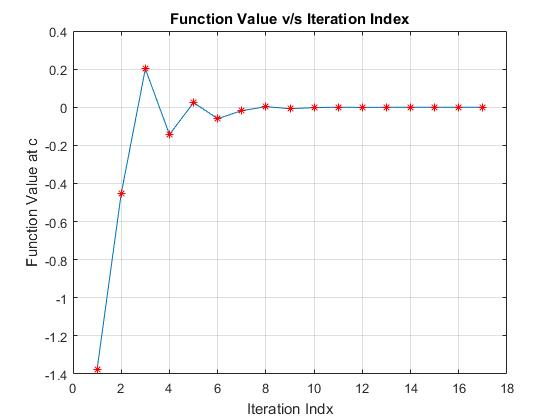
\includegraphics[scale = 0.36]{x3-x2-x-1_value_1.jpg}
    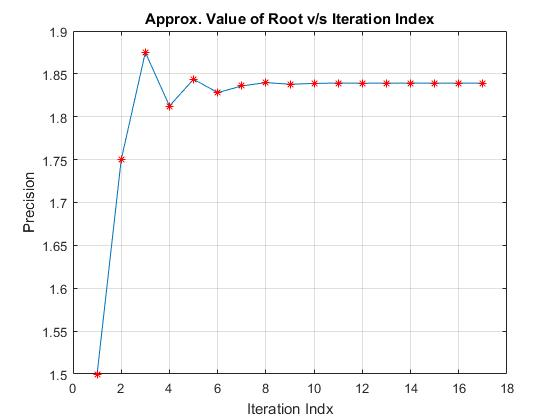
\includegraphics[scale = 0.36]{x3-x2-x-1_1_root.jpg}
    \caption{Fig 1.1,1.2 : Positive root of $x^3 - x^2 -x-1 = 0$}
    \label{fig:ques2}
\end{figure}
\subsection{Tables}
\begin{table}[!h]
\centering{\Large
\begin{tabular}{|c|c|c|c|c|c|c|c|}\hline
ItrNo & a      & b      & c      & f(c)    & f(a)*f(c) & a-c=b-c & Assign\\ \hline
1  & 1      & 2      & 1.5    & -1.375  & >0  & 0.5 & Set a=c   \\
2  & 1.5    & 2      & 1.75   & -0.4531 & >0 & 0.25 & Set a=c  \\
3  & 1.75   & 2      & 1.875  & 0.2012  & <0 & 0.125  & Set b=c\\
4  & 1.75   & 1.875  & 1.8125 & -0.1433 & >0 & 0.0625 & Set a=c\\
5  & 1.8125 & 1.875  & 1.8438 & 0.0245  & <0 & 0.0313 & Set b=c\\
6  & 1.8125 & 1.8438 & 1.8281 & -0.0605 & >0 & 0.0156 & Set a=c\\
7  & 1.8281 & 1.8438 & 1.8359 & -0.0183 & >0 & 0.0078 & Set a=c\\
8  & 1.8359 & 1.8438 & 1.8398 & 0.003   & <0 & 0.0039 & Set b=c\\
9  & 1.8359 & 1.8398 & 1.8379 & -0.0076 & >0 & 0.002  & Set a=c\\
10 & 1.8379 & 1.8398 & 1.8389 & -0.0023 & >0 & 0.001  & Set a=c\\
11 & 1.8389 & 1.8398 & 1.8394 & 0.0004  & <0 & 0.0005 & Set b=c\\
12 & 1.8389 & 1.8394 & 1.8391 & -0.001  & >0 & 0.0002 & Set a=c\\
13 & 1.8391 & 1.8394 & 1.8392 & -0.0003 & >0 & 0.0001 & Set a=c\\
14 & 1.8392 & 1.8394 & 1.8393 & 0       & <0 & 0.0001 & Set b=c\\
\hline
\end{tabular}}
\caption{Positive Root of $x^3 - x^2 - x - 1 =0$}
\end{table}

\newpage
\section{$f(x) = 1 +0.3cos(x) - x$}

From a rough plot of the function, we can see that there can exist only one intersection between the curves, $f_1(x) = 0.3\cos{x} + 1$ and $f_2(x) = x$. At $x = 0$, $f(x) = 1.3$ and at $x = \frac{\pi}{2}$, $f(x) = 1-\frac{\pi}{2} < 0$.
\subsection{Plots}
\begin{figure}[!h]
    \centering
    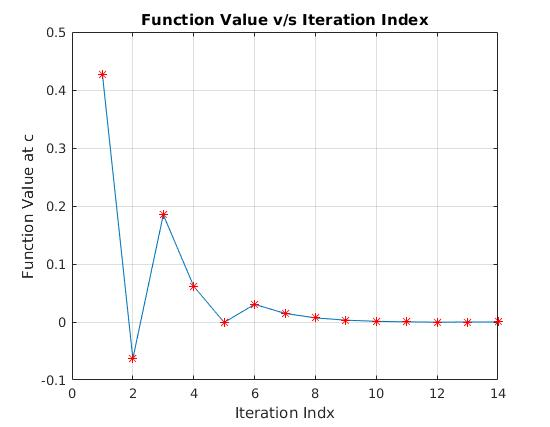
\includegraphics[scale = 0.4]{1plus03cosx-x_value.jpg}
    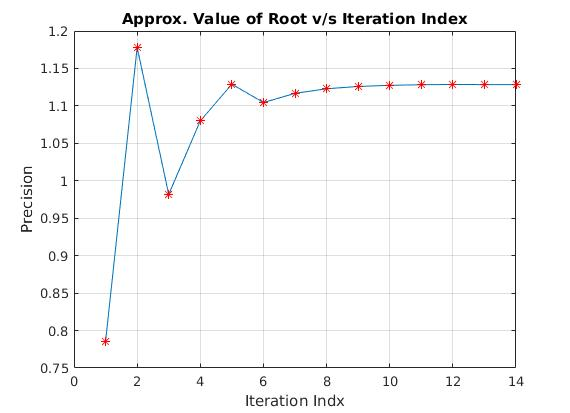
\includegraphics[scale = 0.4]{1plus03cosx-x_root.jpg}
    \caption{Fig 1.1,1.2 : Positive root of $f(x) = 1 +0.3cos(x) - x$}
    \label{fig:ques3}
\end{figure}
\subsection{Tables}
\begin{table}[!h]
\centering{\Large
\begin{tabular}{|c|c|c|c|c|c|c|c|}\hline
ItrNo & a      & b      & c      & f(c)    & f(a)*f(c) & a-c=b-c & Assign\\ \hline
1  & 0       & 1.5708 & 0.7854  & 0.42673  & \textgreater{}0 & 0.7854  & Set a=c\\
2  & 0.7854  & 1.5708 & 1.1781  & -0.06329 & \textless{}0    & 0.3927  & Set b=c\\
3  & 0.7854  & 1.1781 & 0.98175 & 0.18492  & \textgreater{}0 & 0.19635 & Set a=c\\
4  & 0.98175 & 1.1781 & 1.0799  & 0.0615   & \textgreater{}0 & 0.09817 & Set a=c\\
5  & 1.0799  & 1.1781 & 1.129   & -0.00074 & \textless{}0    & 0.04909 & Set b=c\\
6  & 1.0799  & 1.129  & 1.1045  & 0.03042  & \textgreater{}0 & 0.02454 & Set a=c\\
7  & 1.1045  & 1.129  & 1.1167  & 0.01485  & \textgreater{}0 & 0.01227 & Set a=c\\
8  & 1.1167  & 1.129  & 1.1229  & 0.00705  & \textgreater{}0 & 0.00614 & Set a=c\\
9  & 1.1229  & 1.129  & 1.1259  & 0.00316  & \textgreater{}0 & 0.00307 & Set a=c\\
10 & 1.1259  & 1.129  & 1.1275  & 0.00121  & \textgreater{}0 & 0.00153 & Set a=c\\
11 & 1.1275  & 1.129  & 1.1282  & 0.00023  & \textgreater{}0 & 0.00077 & Set a=c\\
12 & 1.1282  & 1.129  & 1.1286  & -0.00026 & \textless{}0    & 0.00038 & Set b=c\\
13 & 1.1282  & 1.1286 & 1.1284  & -1e-05   & \textless{}0    & 0.00019 & Set b=c\\
14 & 1.1282  & 1.1284 & 1.1283  & 0.00011  & \textgreater{}0 & 0.0001  & Set a=c\\
\hline
\end{tabular}}
\caption{Positive Root of $f(x) = 1 +0.3cos(x) - x$}
\end{table}
\newpage



\section{$f(x) = 0.5 + \sin{x} - \cos{x}$}
We see that at $x = 0$, $f_1(x) = 0.5+\sin{x} = 0.5$ and $f_2(x) = \cos{x} = 1$. And at $x = \frac{\pi}{2}$, $f_1{\frac{\pi}{2}} = 1.5$ and $f_2(x) = 0$. Note that the functions $f_1(x)$ and $f_2(x)$ are monotonic between $x = 0$ and $x = \frac{\pi}{2}$ so there can't be any other intersection between the two.
\subsection{Plots}
\begin{figure}[!h]
    \centering
    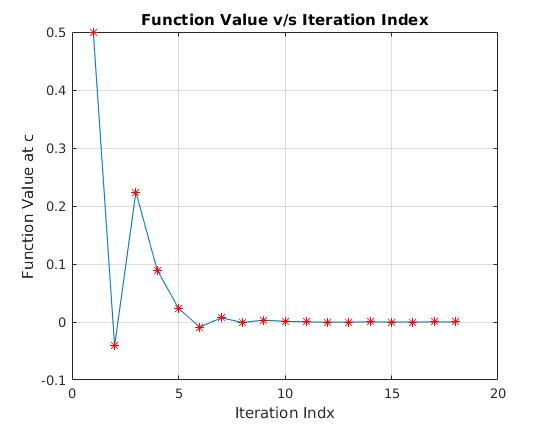
\includegraphics[scale = 0.4]{05-cosplussin_value.jpg}
    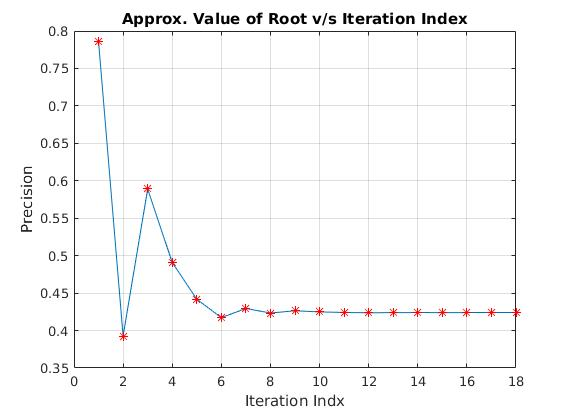
\includegraphics[scale = 0.4]{05-cosplussin_root.jpg}
    \caption{Fig 1.1,1.2 : Positive root of $f(x) = 0.5 + \sin{x} - \cos{x}$}
    \label{fig:ques4}
\end{figure}
\subsection{Tables}
\begin{table}[!h]
\centering{\Large
\begin{tabular}{|c|c|c|c|c|c|c|c|}\hline
ItrNo & a      & b      & c      & f(c)    & f(a)*f(c) & a-c=b-c & Assign\\ \hline
1  & 0       & 1.5708  & 0.7854  & 0.5     & <0 & 0.7854 & Set b=c\\
2  & 0       & 0.7854  & 0.3927  & -0.0412 & >0  & 0.3927 & Set a=c\\
3  & 0.3927  & 0.7854  & 0.589   & 0.2241  & <0 & 0.1963 & Set b=c\\
4  & 0.3927  & 0.589   & 0.4909  & 0.0895  & <0 & 0.0982 & Set b=c\\
5  & 0.3927  & 0.4909  & 0.4418  & 0.0236  & <0 & 0.0491 & Set b=c\\
6  & 0.3927  & 0.4418  & 0.4172  & -0.009  & >0  & 0.0245 & Set a=c\\
7  & 0.4172  & 0.4418  & 0.4295  & 0.0073  & <0 & 0.0123 & Set b=c\\
8  & 0.4172  & 0.4295  & 0.4234  & -0.0009 & >0 & 0.0061 & Set a=c\\
9  & 0.4234  & 0.4295  & 0.4264  & 0.0032  & <0 & 0.0031 & Set b=c\\
10 & 0.4234  & 0.4264  & 0.4249  & 0.0012  & <0 & 0.0015 & Set b=c\\
11 & 0.4234  & 0.4249  & 0.4241  & 0.0002  & <0 & 0.0008 & Set b=c\\
12 & 0.4234  & 0.4241  & 0.4238  & -0.0004 & >0  & 0.0004 & Set a=c\\
13 & 0.4238  & 0.4241  & 0.424   & -0.0001 & >0 & 0.0002 & Set a=c\\
14 & 0.424   & 0.4241  & 0.424   & 0       & <0 & 0.0001 & Set b=c\\
\hline
\end{tabular}}
\caption{The smallest Positive Root of $f(x) = 0.5 + \sin{x} - \cos{x}$}
\end{table}
\newpage



\section{$f(x) = x - e^{-x}$}
Note that the function $f_1(x) = e^{-x}$ is monotonically decreasing and $f_2(x) = x$ is monotonically increasing. Hence there exist only one root. At $x = 0$, $f(x) = -1$ and at $x = 1$, $f(x) = 0$. Hence the root lies between these two values. 
\subsection{Plots}
\begin{figure}[!h]
    \centering
    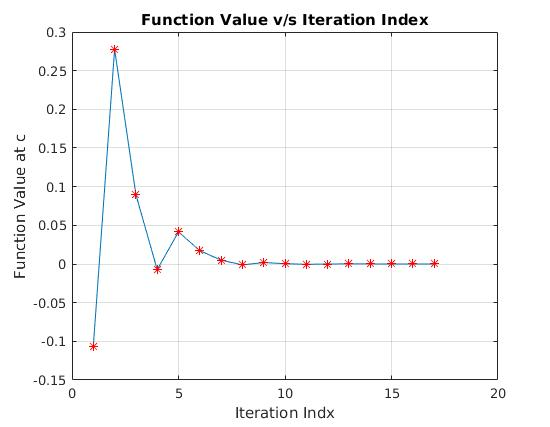
\includegraphics[scale = 0.4]{x-ex_value.jpg}
    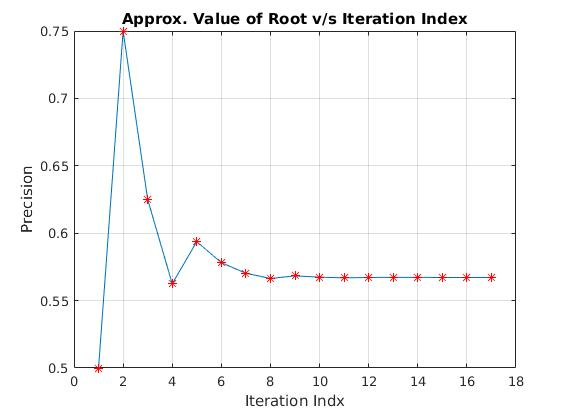
\includegraphics[scale = 0.4]{x-ex_root.jpg}
    \caption{Fig 1.1,1.2 : Positive root of $f(x) = x - - e^{-x}$}
    \label{fig:ques5}
\end{figure}
\subsection{Tables}
\begin{table}[!h]
\centering{\Large
\begin{tabular}{|c|c|c|c|c|c|c|c|}\hline
ItrNo & a      & b      & c      & f(c)    & f(a)*f(c) & a-c=b-c & Assign\\ \hline
1  & 0      & 1      & 0.5    & -0.1065 & >0  & 0.5   & Set a=c \\
2  & 0.5    & 1      & 0.75   & 0.2776  & <0 & 0.25   & Set b=c\\
3  & 0.5    & 0.75   & 0.625  & 0.0897  & <0 & 0.125  & Set b=c\\
4  & 0.5    & 0.625  & 0.5625 & -0.0073 & >0 & 0.0625 & Set a=c\\
5  & 0.5625 & 0.625  & 0.5938 & 0.0415  & <0 & 0.0313 & Set b=c\\
6  & 0.5625 & 0.5938 & 0.5781 & 0.0172  & <0 & 0.0156 & Set b=c\\
7  & 0.5625 & 0.5781 & 0.5703 & 0.005   & <0 & 0.0078 & Set b=c\\
8  & 0.5625 & 0.5703 & 0.5664 & -0.0012 & >0 & 0.0039 & Set a=c\\
9  & 0.5664 & 0.5703 & 0.5684 & 0.0019  & <0 & 0.002  & Set b=c\\
10 & 0.5664 & 0.5684 & 0.5674 & 0.0004  & <0 & 0.001  & Set b=c\\
11 & 0.5664 & 0.5674 & 0.5669 & -0.0004 & >0  & 0.0005 & Set a=c\\
12 & 0.5669 & 0.5674 & 0.5671 & 0       & >0 & 0.0002 & Set a=c\\
13 & 0.5671 & 0.5674 & 0.5673 & 0.0002  & <0 & 0.0001 & Set b=c\\
14 & 0.5671 & 0.5673 & 0.5672 & 0.0001  & <0 & 0.0001 & Set b=c\\
\hline
\end{tabular}}
\caption{The smallest Positive Root of $f(x) = x - e^{-x}$}
\end{table}
\newpage


\section{$f(x) = \sin{x} - e^{-x}$}
At $x = 0$, the values of $f_2(x) = e^{-x}$ enter the range of values of $f_1(x) = \sin{x}$ with $f(x) = -1$. At $x = \frac{\pi}{2}$, $f(x) > 0$. Between 0 and $\frac{\pi}{2}$, both the functions are monotonic. Hence there can exist only one root between the two values.
\newline
The second root occurs when $f_2(x) = e^{-x}$ cuts $f_1(x) = \sin{x}$ in the first lobe for the second time. The first time being between $0 < < \frac{pi}{2}$ and the second time being between $\frac{pi}{2} < x <\pi$.
\subsection{Plots}
\begin{figure}[!h]
    \centering
    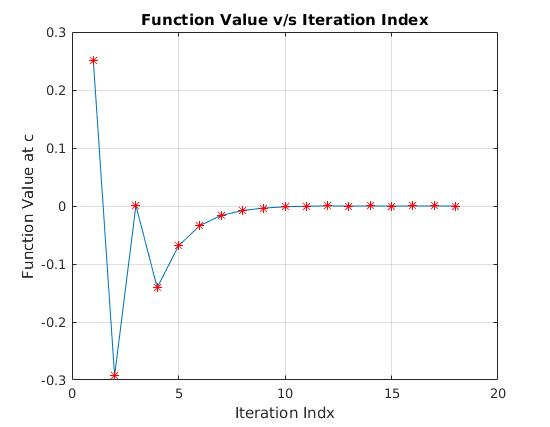
\includegraphics[scale = 0.4]{e-x-sinx_value1.jpg}
    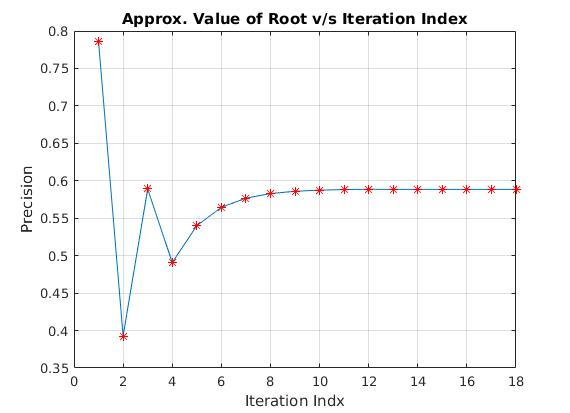
\includegraphics[scale = 0.4]{e-x-sinx_root1.jpg}
    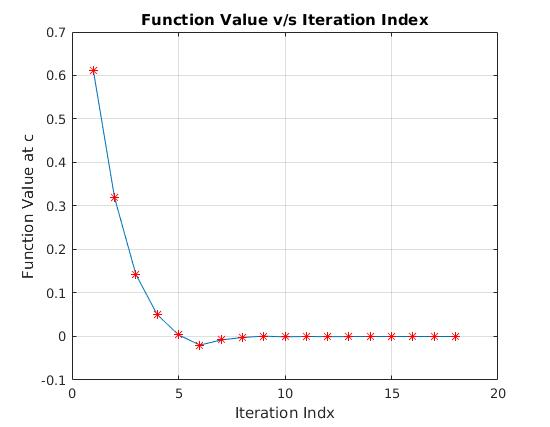
\includegraphics[scale = 0.4]{e-x-sinx_value2.jpg}
    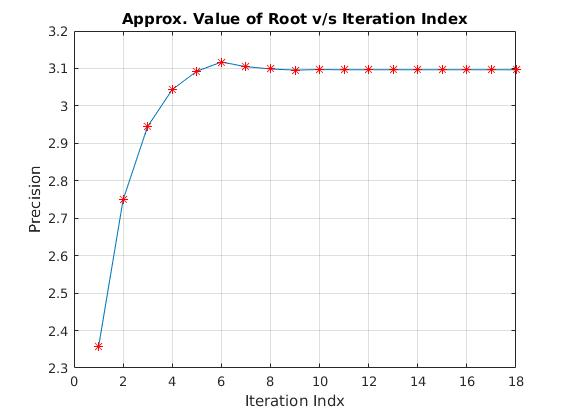
\includegraphics[scale = 0.4]{e-x-sinx_root2.jpg}
    \caption{Fig 1.1,1.2 : First smallest Positive root of $f(x) = \sin{x} - e^{-x}$ 
     || Fig 1.3,1.4 : Second Smallest Positive root of $f(x) = \sin{x} - e^{-x}$}
    \label{fig:ques6}
\end{figure}
\newpage
\subsection{Tables}
\begin{table}[!h]
\centering{\Large
\begin{tabular}{|c|c|c|c|c|c|c|c|}\hline
ItrNo & a      & b      & c      & f(c)    & f(a)*f(c) & a-c=b-c & Assign\\ \hline
1  & 0      & 1.5708 & 0.7854 & 0.2512  & <0 & 0.7854 & Set b=c\\
2  & 0      & 0.7854 & 0.3927 & -0.2925 & >0 & 0.3927 & Set a=c\\
3  & 0.3927 & 0.7854 & 0.589  & 0.0007  & <0 & 0.1963 & Set b=c\\
4  & 0.3927 & 0.589  & 0.4909 & -0.1407 & >0  & 0.0982 & Set a=c\\
5  & 0.4909 & 0.589  & 0.54   & -0.0687 & >0 & 0.0491 & Set a=c\\
6  & 0.54   & 0.589  & 0.5645 & -0.0336 & >0 & 0.0245 & Set a=c\\
7  & 0.5645 & 0.589  & 0.5768 & -0.0164 & >0 & 0.0123 & Set a=c\\
8  & 0.5768 & 0.589  & 0.5829 & -0.0078 & >0 & 0.0061 & Set a=c\\
9  & 0.5829 & 0.589  & 0.586  & -0.0035 & >0 & 0.0031 & Set a=c\\
10 & 0.586  & 0.589  & 0.5875 & -0.0014 & >0 & 0.0015 & Set a=c\\
11 & 0.5875 & 0.589  & 0.5883 & -0.0003 & >0 & 0.0008 & Set a=c\\
12 & 0.5883 & 0.589  & 0.5887 & 0.0002  & <0 & 0.0004 & Set b=c\\
13 & 0.5883 & 0.5887 & 0.5885 & -0.0001 & >0 & 0.0002 & Set a=c\\
14 & 0.5885 & 0.5887 & 0.5886 & 0.0001  & <0 & 0.0001 & Set b=c\\
\hline
\end{tabular}}
\caption{The first smallest Positive Root of $f(x) = \sin{x} - e^{-x}$}
\end{table}
\begin{table}[!h]
\centering{\Large
\begin{tabular}{|c|c|c|c|c|c|c|c|}\hline
ItrNo & a      & b      & c      & f(c)    & f(a)*f(c) & a-c=b-c & Assign \\ \hline
1  & 1.5708 & 3.1416 & 2.3562 & 0.6123  & >0  & 0.7854 & Set a=c\\
2  & 2.3562 & 3.1416 & 2.7489 & 0.3187  & >0  & 0.3927 & Set a=c\\
3  & 2.7489 & 3.1416 & 2.9452 & 0.1425  & >0  & 0.1963 & Set a=c\\
4  & 2.9452 & 3.1416 & 3.0434 & 0.0503  & >0  & 0.0982 & Set a=c\\
5  & 3.0434 & 3.1416 & 3.0925 & 0.0037  & >0  & 0.0491 & Set a=c\\
6  & 3.0925 & 3.1416 & 3.117  & -0.0197 & <0 & 0.0245 & Set b=c\\
7  & 3.0925 & 3.117  & 3.1048 & -0.008  & <0 & 0.0123 & Set b=c\\
8  & 3.0925 & 3.1048 & 3.0986 & -0.0022 & <0 & 0.0061 & Set b=c\\
9  & 3.0925 & 3.0986 & 3.0956 & 0.0008  & >0  & 0.0031 & Set a=c\\
10 & 3.0956 & 3.0986 & 3.0971 & -0.0007 & <0 & 0.0015 & Set b=c\\
11 & 3.0956 & 3.0971 & 3.0963 & 0       & >0  & 0.0008 & Set a=c\\
12 & 3.0963 & 3.0971 & 3.0967 & -0.0003 & <0 & 0.0004 & Set b=c\\
13 & 3.0963 & 3.0967 & 3.0965 & -0.0002 & <0 & 0.0002 & Set b=c\\
14 & 3.0963 & 3.0965 & 3.0964 & -0.0001 & <0 & 0.0001 & Set b=c\\
\hline
\end{tabular}}
\caption{The Second smallest Positive Root of $f(x) = \sin{x} - e^{-x}$}
\end{table}
\newpage




\section{$f(x) = x^3 -2x -2$}
We have $f'(x) = 3x^2-2$. Hence the local maxima lies at $x = -\sqrt{\frac{2}{3}}$ and at this point $f(-\sqrt{\frac{2}{3}}) < 0$, so there is only root of this equation. At $x = 1$, $f(x) = -3$ and at $x = 2$, $f(x) = 2$. Hence the only real root of $f(x)$ lies between 1 and 2.
\subsection{Plots}
\begin{figure}[!h]
    \centering
    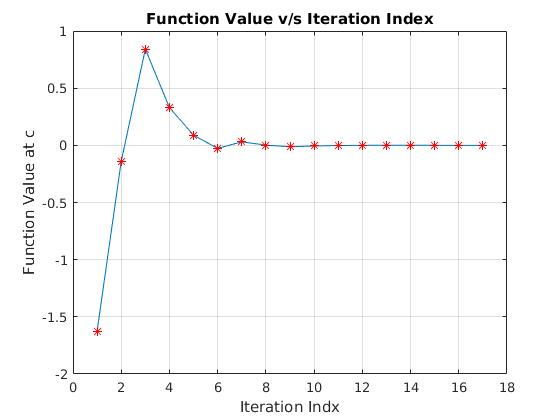
\includegraphics[scale = 0.4]{x3-2x-2_value.jpg}
    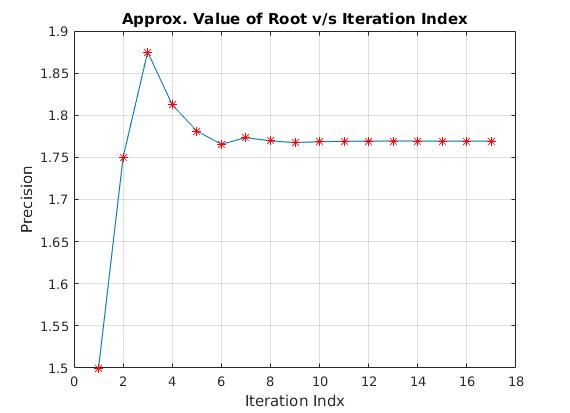
\includegraphics[scale = 0.4]{x3-2x-2_root.jpg}
    %\caption{Fig 1.1,1.2 :Positive root of $f(x) = x^3 -2x -2$ }
    \label{fig:ques7}
\end{figure}
\subsection{Tables}
\begin{table}[!h]
\centering{\Large
\begin{tabular}{|c|c|c|c|c|c|c|c|}\hline
ItrNo & a      & b      & c      & f(c)    & f(a)*f(c) & a-c=b-c & Assign\\ \hline
1  & 1      & 2      & 1.5    & -1.625  & >0  & 0.5   & Set a=c \\
2  & 1.5    & 2      & 1.75   & -0.1406 & >0  & 0.25   & Set a=c\\
3  & 1.75   & 2      & 1.875  & 0.8418  & <0 & 0.125  & Set b=c\\
4  & 1.75   & 1.875  & 1.8125 & 0.3293  & <0 & 0.0625 & Set b=c\\
5  & 1.75   & 1.8125 & 1.7813 & 0.0891  & <0 & 0.0313 & Set b=c\\
6  & 1.75   & 1.7813 & 1.7656 & -0.027  & >0 & 0.0156 & Set a=c\\
7  & 1.7656 & 1.7813 & 1.7734 & 0.0307  & <0 & 0.0078 & Set b=c\\
8  & 1.7656 & 1.7734 & 1.7695 & 0.0018  & <0 & 0.0039 & Set b=c\\
9  & 1.7656 & 1.7695 & 1.7676 & -0.0127 & >0 & 0.002  & Set a=c\\
10 & 1.7676 & 1.7695 & 1.7686 & -0.0054 & >0 & 0.001  & Set a=c\\
11 & 1.7686 & 1.7695 & 1.769  & -0.0018 & >0 & 0.0005 & Set a=c\\
12 & 1.769  & 1.7695 & 1.7693 & 0       & >0 & 0.0002 & Set a=c\\
13 & 1.7693 & 1.7695 & 1.7694 & 0.0009  & <0 & 0.0001 & Set b=c\\
14 & 1.7693 & 1.7694 & 1.7693 & 0.0004  & <0 & 0.0001 & Set b=c\\
\hline
\end{tabular}}
\caption{The Positive Root of $f(x) = x^3 -2x -2$}
\end{table}



\newpage
\section{$f(x) = x^4 -x -1$}
Graphically, we can see that there are only 2 roots of this equation since $f_1(x) = x^4$ and $f_2(x) = x+1$ cut in only 2 points, once in positive x-axis and once in negative x-axis.
\newline
\newline
At $x = 1$, $f(x) = -1$ and at $x = 2$, $f(x) = 13$. Hence the positive root lies between 1 and 2. Again t $x = 0$, $f(x) = -1$ and at $x = -1$, $f(x) = 1$. Hence the negative root lies between -1 and 0.
\subsection{Plots}
\begin{figure}[!h]
    \centering
    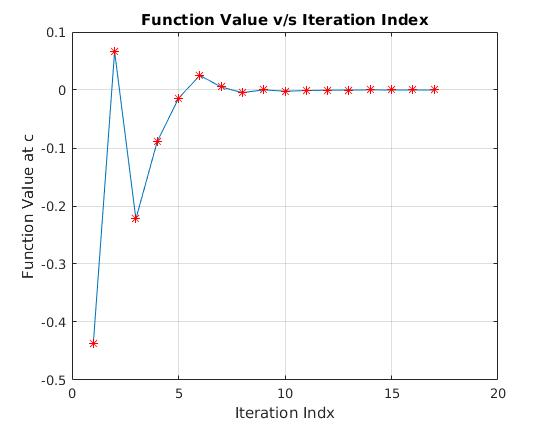
\includegraphics[scale = 0.4]{x4-x-1_value1.jpg}
    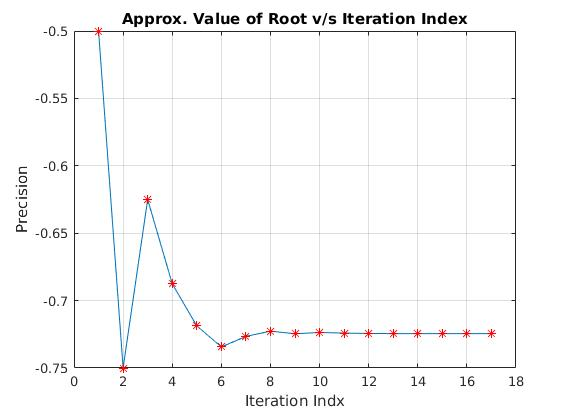
\includegraphics[scale = 0.4]{x4-x-1_root1.jpg}
    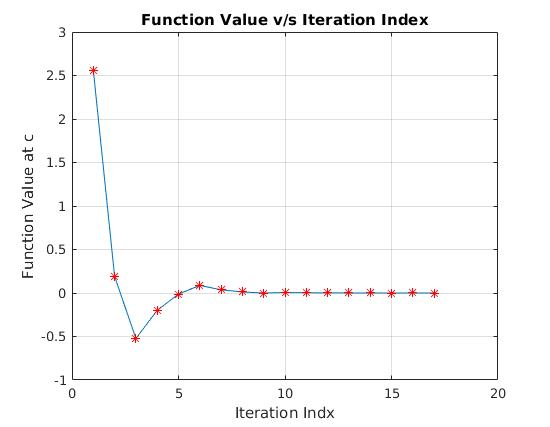
\includegraphics[scale = 0.4]{x4-x-1_value2.jpg}
    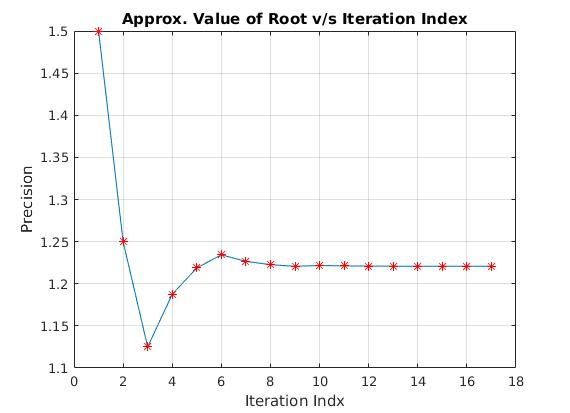
\includegraphics[scale = 0.4]{x4-x-1_root2.jpg}
    \caption{Fig 1.1,1.2 : Negative root of $f(x) = x^4 -x -1$ 
     || Fig 1.3,1.4 : Positive root of $f(x) = x^4 -x -1$}
    \label{fig:ques8}
\end{figure}\newpage
\subsection{Tables}
\begin{table}[!h]
\centering{\Large
\begin{tabular}{|c|c|c|c|c|c|c|c|}\hline
ItrNo & a      & b      & c      & f(c)    & f(a)*f(c) & a-c=b-c & Assign\\ \hline
1  & 1      & 2      & 1.5    & 2.5625  & <0 & 0.5    & Set b=c\\
2  & 1      & 1.5    & 1.25   & 0.1914  & <0 & 0.25   & Set b=c\\
3  & 1      & 1.25   & 1.125  & -0.5232 & >0 & 0.125  & Set a=c\\
4  & 1.125  & 1.25   & 1.1875 & -0.199  & >0 & 0.0625 & Set a=c\\
5  & 1.1875 & 1.25   & 1.2188 & -0.0125 & >0 & 0.0313 & Set a=c\\
6  & 1.2188 & 1.25   & 1.2344 & 0.0872  & <0 & 0.0156 & Set b=c\\
7  & 1.2188 & 1.2344 & 1.2266 & 0.0368  & <0 & 0.0078 & Set b=c\\
8  & 1.2188 & 1.2266 & 1.2227 & 0.012   & <0 & 0.0039 & Set b=c\\
9  & 1.2188 & 1.2227 & 1.2207 & -0.0003 & >0 & 0.002  & Set a=c\\
10 & 1.2207 & 1.2227 & 1.2217 & 0.0059  & <0 & 0.001  & Set b=c\\
11 & 1.2207 & 1.2217 & 1.2212 & 0.0028  & <0 & 0.0005 & Set b=c\\
12 & 1.2207 & 1.2212 & 1.2209 & 0.0013  & <0 & 0.0002 & Set b=c\\
13 & 1.2207 & 1.2209 & 1.2208 & 0.0005  & <0 & 0.0001 & Set b=c\\
14 & 1.2207 & 1.2208 & 1.2208 & 0.0001  & <0 & 0.0001 & Set b=c\\
\hline
\end{tabular}}
\caption{The Positive Root of $f(x) = x^4 -x -1$}
\end{table}
\begin{table}[!h]
\centering{\Large
\begin{tabular}{|c|c|c|c|c|c|c|c|}\hline
ItrNo & a      & b      & c      & f(c)    & f(a)*f(c) & a-c=b-c & Assign\\ \hline
1  & -1      & 0       & -0.5    & -0.4375 & <0 & 0.5   & Set b=c \\
2  & -1      & -0.5    & -0.75   & 0.0664  & >0 & 0.25  & Set a=c \\
3  & -0.75   & -0.5    & -0.625  & -0.2224 & <0 & 0.125  & Set b=c\\
4  & -0.75   & -0.625  & -0.6875 & -0.0891 & <0 & 0.0625 & Set b=c\\
5  & -0.75   & -0.6875 & -0.7188 & -0.0144 & <0 & 0.0313 & Set b=c\\
6  & -0.75   & -0.7188 & -0.7344 & 0.0252  & >0 & 0.0156 & Set a=c\\
7  & -0.7344 & -0.7188 & -0.7266 & 0.0052  & >0 & 0.0078 & Set a=c\\
8  & -0.7266 & -0.7188 & -0.7227 & -0.0046 & <0 & 0.0039 & Set b=c\\
9  & -0.7266 & -0.7227 & -0.7246 & 0.0003  & >0 & 0.002  & Set a=c\\
10 & -0.7246 & -0.7227 & -0.7236 & -0.0022 & <0 & 0.001  & Set b=c\\
11 & -0.7246 & -0.7236 & -0.7241 & -0.0009 & <0 & 0.0005 & Set b=c\\
12 & -0.7246 & -0.7241 & -0.7244 & -0.0003 & <0 & 0.0002 & Set b=c\\
13 & -0.7246 & -0.7244 & -0.7245 & 0       & <0 & 0.0001 & Set b=c\\
14 & -0.7246 & -0.7245 & -0.7245 & 0.0001  & >0 & 0.0001 & Set a=c\\
\hline
\end{tabular}}
\caption{The Negative Root of $f(x) = x^4 -x -1$}
\end{table}



\newpage
\section{$f(x) = e^x -x -2$}
The functions $f_1(x) = e^x$ and $f_2(x) = x+2$ intersect at only one point. At $x = 1$ at which $f(1) = e-3 < 0$ and at $x = 2$ at which $f(2) = e^2 > 0$. Hence the only real root of this equation lies between 1 and 2.
\subsection{Plots}
\begin{figure}[!h]
    \centering
    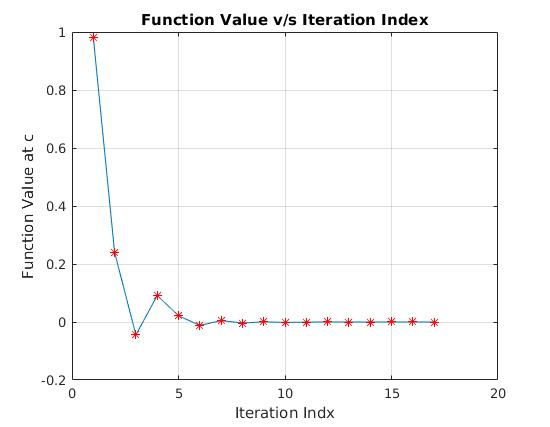
\includegraphics[scale = 0.4]{ex-x-2_value.jpg}
    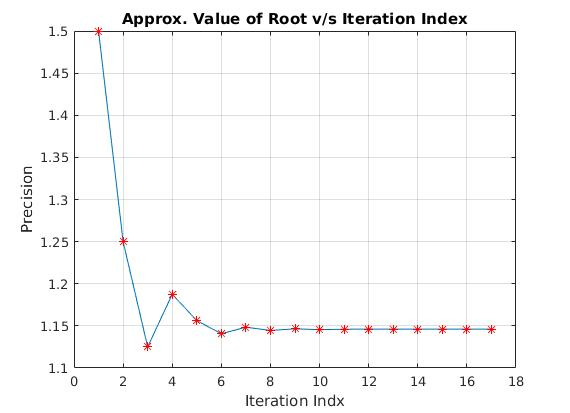
\includegraphics[scale = 0.4]{ex-x-2_root.jpg}
    \caption{Fig 1.1,1.2 :Positive root of $f(x) = e^x -x -2$ }
    \label{fig:ques9}
\end{figure}
\subsection{Tables}
\begin{table}[!h]
\centering{\Large
\begin{tabular}{|c|c|c|c|c|c|c|c|}\hline
ItrNo & a      & b      & c      & f(c)    & f(a)*f(c) & a-c=b-c & Assign \\ \hline
1  & 1      & 2      & 1.5    & 0.9817  & <0 & 0.5   & Set b=c \\
2  & 1      & 1.5    & 1.25   & 0.2403  & <0 & 0.25  & Set b=c \\
3  & 1      & 1.25   & 1.125  & -0.0448 & >0 & 0.125  & Set a=c\\
4  & 1.125  & 1.25   & 1.1875 & 0.0914  & <0 & 0.0625 & Set b=c\\
5  & 1.125  & 1.1875 & 1.1563 & 0.0217  & <0 & 0.0313 & Set b=c\\
6  & 1.125  & 1.1563 & 1.1406 & -0.0119 & >0 & 0.0156 & Set a=c\\
7  & 1.1406 & 1.1563 & 1.1484 & 0.0048  & <0 & 0.0078 & Set b=c\\
8  & 1.1406 & 1.1484 & 1.1445 & -0.0036 & >0 & 0.0039 & Set a=c\\
9  & 1.1445 & 1.1484 & 1.1465 & 0.0006  & <0 & 0.002  & Set b=c\\
10 & 1.1445 & 1.1465 & 1.1455 & -0.0015 & >0 & 0.001  & Set a=c\\
11 & 1.1455 & 1.1465 & 1.146  & -0.0004 & >0 & 0.0005 & Set a=c\\
12 & 1.146  & 1.1465 & 1.1462 & 0.0001  & <0 & 0.0002 & Set b=c\\
13 & 1.146  & 1.1462 & 1.1461 & -0.0002 & >0  & 0.0001 & Set a=c\\
14 & 1.1461 & 1.1462 & 1.1462 & 0       & >0 & 0.0001 & Set a=c\\
\hline
\end{tabular}}
\caption{The Positive Root of $f(x) = e^x -x -2$}
\end{table}



\newpage
\section{$f(x) = 1 -x +\sin{x}$}
Graphically it is easy to see that $f_1(x) = x-1$ and $f_2(x) = \sin{x}$ would intersect in only one point. At $x = \frac{\pi}{2}$, $f(x) = 1-\frac{\pi}{2} < 0$ and at $x = pi$, $f(x) = 2-\pi > 0$. Hence the only root lies between $\frac{\pi}{2}$ and $\pi$. 
\subsection{Plots}
\begin{figure}[!h]
    \centering
    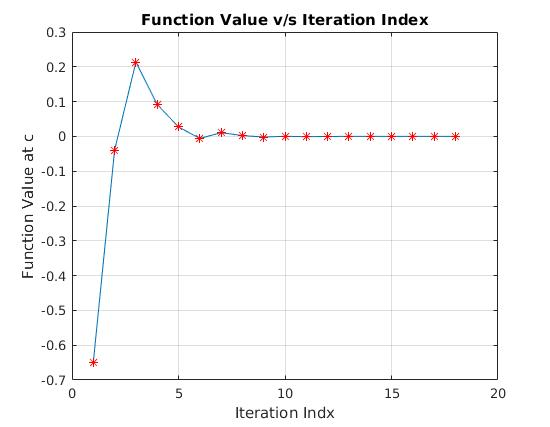
\includegraphics[scale = 0.4]{sinx-xplus1_value.jpg}
    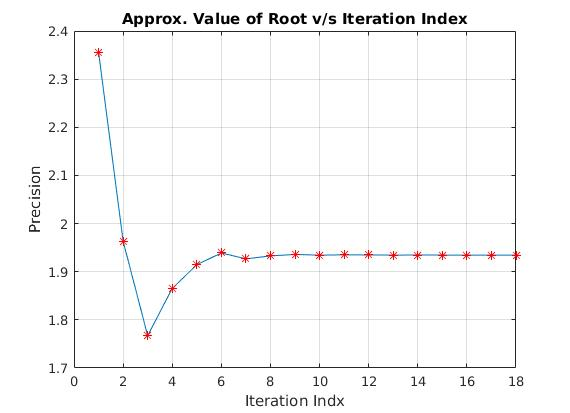
\includegraphics[scale = 0.4]{sinx-xplus1_root.jpg}
    \caption{Fig 1.1,1.2 :Smallest Positive root of $f(x) = 1 -x +\sin{x}$ }
    \label{fig:ques10}
\end{figure}
\subsection{Tables}
\begin{table}[!h]
\centering{\Large
\begin{tabular}{|c|c|c|c|c|c|c|c|}\hline
ItrNo & a      & b      & c      & f(c)    & f(a)*f(c) & a-c=b-c & Assign \\ \hline
1  & 1.5708 & 3.1416 & 2.3562 & -0.6491 & <0 & 0.7854 & Set b=c\\
2  & 1.5708 & 2.3562 & 1.9635 & -0.0396 & <0 & 0.3927 & Set b=c\\
3  & 1.5708 & 1.9635 & 1.7671 & 0.2136  & >0 & 0.1963 & Set a=c\\
4  & 1.7671 & 1.9635 & 1.8653 & 0.0916  & >0 & 0.0982 & Set a=c\\
5  & 1.8653 & 1.9635 & 1.9144 & 0.0271  & >0 & 0.0491 & Set a=c\\
6  & 1.9144 & 1.9635 & 1.939  & -0.006  & <0 & 0.0245 & Set b=c\\
7  & 1.9144 & 1.939  & 1.9267 & 0.0107  & >0 & 0.0123 & Set a=c\\
8  & 1.9267 & 1.939  & 1.9328 & 0.0024  & >0 & 0.0061 & Set a=c\\
9  & 1.9328 & 1.939  & 1.9359 & -0.0018 & <0 & 0.0031 & Set b=c\\
10 & 1.9328 & 1.9359 & 1.9343 & 0.0003  & >0 & 0.0015 & Set a=c\\
11 & 1.9343 & 1.9359 & 1.9351 & -0.0008 & <0 & 0.0008 & Set b=c\\
12 & 1.9343 & 1.9351 & 1.9347 & -0.0002 & <0 & 0.0004 & Set b=c\\
13 & 1.9343 & 1.9347 & 1.9345 & 0       & >0 & 0.0002 & Set a=c\\
14 & 1.9345 & 1.9347 & 1.9346 & -0.0001 & <0 & 0.0001 & Set b=c\\
\hline
\end{tabular}}
\caption{The smallest Positive Root of $f(x) = 1 -x +\sin{x}$}
\end{table}



\newpage
\section{$f(x) = -x +\tan{x}$}
The functions $f_1(x) = x$ and $f_2(x) = \tan{x}$ cut many times however only once in each period of $f_2(x) = \tan{x}$ on account of $\tan{x}$ being monotonic in each period. $x$ cuts $\tan{x}$ in period of $\frac{\pi}{2} < x < \frac{3\pi}{2}$. At $x = 0$, $\tan{x} < x$ and at $x = \frac{3\pi}{2}$ $\tan{x} > x$ so the root lies between these 2 values. 
\newline
However, $\tan{x}$ is undefined at $x = \frac{3\pi}{2}$. So we take a value $x = \frac{3\pi}{2} - \epsilon$ where ideally $\epsilon \to 0$ but computationally can be taken as $\epsilon = 0.00001$ since we want our answer accurate upto the 4th decimal place only.
\newline
As discussed earlier, the roots lie in intervals of $k\pi$ to $\frac{3}{2}k\pi$. So first we find the interval of $x = 100$. We get $k = 31$ since $k = \lfloor \frac{100}{\pi} \rfloor$. 
\subsection{Plots}
\begin{figure}[!h]
    \centering
    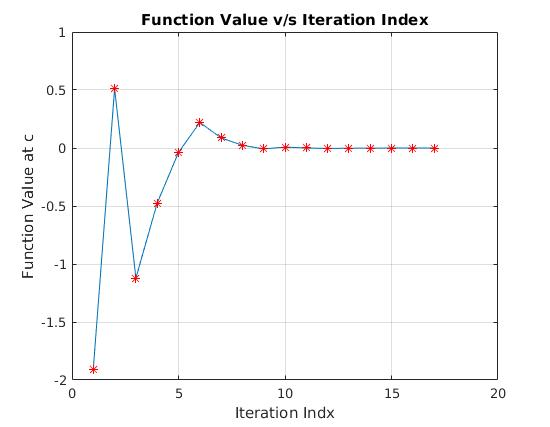
\includegraphics[scale = 0.4]{x-tanx_value.jpg}
    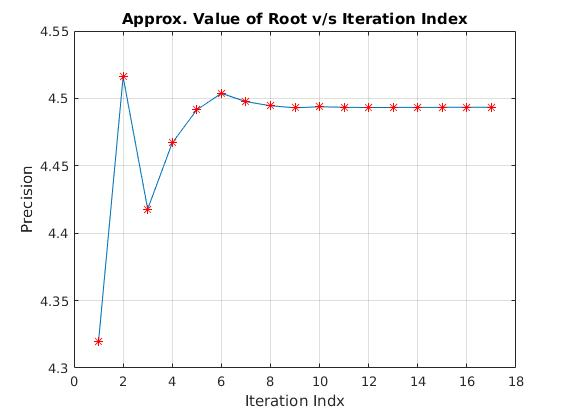
\includegraphics[scale = 0.4]{x-tanx_root.jpg}
    \caption{Fig Smallest Positive root of $f(x) = -x +\tan{x}$ }
    \label{fig:ques11_a}
\end{figure}
\begin{figure}[!h]
    \centering
    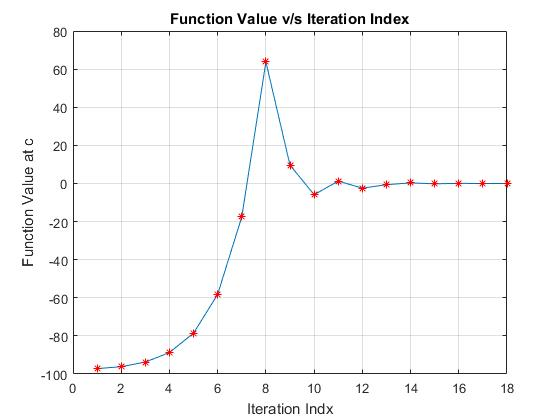
\includegraphics[scale = 0.4]{x-tanx_2_value.jpg}
    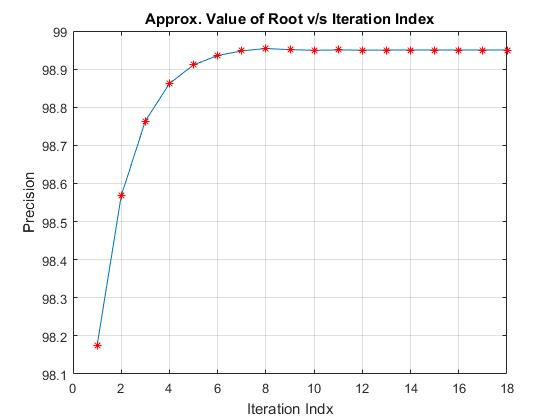
\includegraphics[scale = 0.4]{x-tanx_2_root.jpg}
    \caption{Fig Root of $f(x) = -x +\tan{x}$ near $x = 100$}
    \label{fig:ques11_b}
\end{figure}
\

\begin{table}[!ht]
\centering{\Large
\begin{tabular}{|c|c|c|c|c|c|c|c|}\hline
ItrNo & a      & b      & c      & f(c)    & f(a)*f(c) & a-c=b-c & Assign\\ \hline
1  & 3.1416 & 4.7124 & 3.927  & -2.927  & >0  & 0.7854 & Set a=c\\
2  & 3.927  & 4.7124 & 4.3197 & -1.9055 & >0  & 0.3927 & Set a=c\\
3  & 4.3197 & 4.7124 & 4.516  & 0.5113  & <0 & 0.1963 & Set b=c\\
4  & 4.3197 & 4.516  & 4.4179 & -1.1213 & >0  & 0.0982 & Set a=c\\
5  & 4.4179 & 4.516  & 4.467  & -0.4747 & >0 & 0.0491 & Set a=c\\
6  & 4.467  & 4.516  & 4.4915 & -0.0383 & >0 & 0.0245 & Set a=c\\
7  & 4.4915 & 4.516  & 4.5038 & 0.2199  & <0 & 0.0123 & Set b=c\\
8  & 4.4915 & 4.5038 & 4.4976 & 0.087   & <0 & 0.0061 & Set b=c\\
9  & 4.4915 & 4.4976 & 4.4946 & 0.0234  & <0 & 0.0031 & Set b=c\\
10 & 4.4915 & 4.4946 & 4.493  & -0.0077 & >0 & 0.0015 & Set a=c\\
11 & 4.493  & 4.4946 & 4.4938 & 0.0078  & <0 & 0.0008 & Set b=c\\
12 & 4.493  & 4.4938 & 4.4934 & 0.0001  & <0 & 0.0004 & Set b=c\\
13 & 4.493  & 4.4934 & 4.4932 & -0.0038 & >0 & 0.0002 & Set a=c\\
14 & 4.4932 & 4.4934 & 4.4933 & -0.0019 & >0 & 0.0001 & Set a=c\\
\hline
\end{tabular}}
\caption{The smallest Positive Root of $f(x) = -x +\tan{x}$}
\end{table}
\begin{table}[!ht] %banne table ek page par nai avta?
\centering{\Large
\begin{tabular}{|c|c|c|c|c|c|c|c|}\hline
ItrNo & a      & b      & c      & f(c)    & f(a)*f(c) & a-c=b-c & Assign\\ \hline
1  & 97.389 & 98.96  & 98.175 & -97.175 & >0  & 0.7854 & Set a=c\\
2  & 98.175 & 98.96  & 98.567 & -96.153 & >0 & 0.3927 & Set a=c\\
3  & 98.567 & 98.96  & 98.764 & -93.737 & >0 & 0.1963 & Set a=c\\
4  & 98.764 & 98.96  & 98.862 & -88.71  & >0 & 0.0982 & Set a=c\\
5  & 98.862 & 98.96  & 98.911 & -78.56  & >0 & 0.0491 & Set a=c\\
6  & 98.911 & 98.96  & 98.936 & -58.217 & >0 & 0.0245 & Set a=c\\
7  & 98.936 & 98.96  & 98.948 & -17.531 & >0 & 0.0123 & Set a=c\\
8  & 98.948 & 98.96  & 98.954 & 63.754  & <0 & 0.0061 & Set b=c\\
9  & 98.948 & 98.954 & 98.951 & 9.5785  & <0 & 0.0031 & Set b=c\\
10 & 98.948 & 98.951 & 98.949 & -5.9107 & >0 & 0.0015 & Set a=c\\
11 & 98.949 & 98.951 & 98.95  & 1.2387  & <0 & 0.0008 & Set b=c\\
12 & 98.949 & 98.95  & 98.95  & -2.4683 & >0 & 0.0004 & Set a=c\\
13 & 98.95  & 98.95  & 98.95  & -0.6497 & >0 & 0.0002 & Set a=c\\
14 & 98.95  & 98.95  & 98.95  & 0.2855  & <0 & 0.0001 & Set b=c\\
15 & 98.95  & 98.95  & 98.95  & -0.1843 & >0 & 0      & Set a=c\\
\hline
\end{tabular}}
\caption{The Positive Root of $f(x) = -x +\tan{x}$ around 100}
\end{table}
\end{document}